\section{数据探索与规律发现}

本章把全部可观察到的数据规律逐一列出\nobreak，并\textbf{逐条给出建模决策}\nobreak：能够带来成本改进的规律
显式写入模型（第 5--8 节\nobreak）\nobreak；不单独建模的规律同样给出“数据 + 图表\nobreak”的理由\nobreak，避免“拍脑袋取舍\nobreak”\nobreak。

\subsection{数据总览与质量核验}

\begin{table}[htbp]
\centering
\caption{数据质量核验结果（清洗前后\nobreak）}
\label{tab:quality}
\zihao{-5}
\begin{tabular}{@{}lllll@{}}
\toprule
数据 & 原始形态 & 缺失 & 负值/重复 & 清洗后 \\
\midrule
附件1 & 144$\times$4（区间结束时刻标签\nobreak） & 0 & 0 / 0 & 长表 144 行（slot 1--144\nobreak） \\
附件2 负载 & 365$\times$145（宽表\nobreak） & 0 & 0 / 0 & 长表 52\,560 行 \\
附件2 光伏 & 365$\times$145 & 0 & 0 / 0 & 长表 52\,560 行 \\
附件3 预报 & 1460$\times$26 & 1095（结构空值\nobreak） & 0 / 0 & 向下填充\nobreak；35040 行绝对小时映射 \\
附件4 电价 & 365$\times$145 & 0 & 0 / 0 & 长表 52\,560 行 \\
\bottomrule
\end{tabular}
\end{table}

统一时间轴为 $(date,slot)$\nobreak：日期取 2025-01-01 至 12-31 共 365 天\nobreak，$slot=1,\dots,144$
对应区间 $[(slot-1)\times10,\,slot\times10)$ 分钟\nobreak。功率（kW\nobreak）与电量（kWh\nobreak）的换算是
$1\ \text{kWh}=\text{kW}\times\frac{10}{60}\ \text{h}$\nobreak。附件3 的预报口径经实测校验为
“发布时刻后第 $k$ 个整点的功率点\nobreak”（如 0:00 发布的“预报 7 小时\nobreak”=3.12 kW 对应 7:00 实测 3.08 kW\nobreak）\nobreak，
故用\textbf{整点功率点 + 线性插值}细化到 10 分钟\nobreak。

\subsection{规律一\nobreak：周内负荷规律（周五\nobreak、周六显著偏低\nobreak）}

按星期统计日均用电量\nobreak：周一至周四与周日均为 123.9--124.9 MWh/日\nobreak，而\textbf{周五 78.3 MWh\nobreak、
周六 78.4 MWh\nobreak，比其他五天低 36.8\%}（\cref{fig:weekly} 左上\nobreak）\nobreak。该规律在 12 个月中全部成立\nobreak，
是“昨日外推\nobreak”预测的最大误差来源\nobreak：若用周四实测预测周五\nobreak，负荷被系统性高估约 46\%\nobreak。

\textbf{建模决策（已建模\nobreak，并进一步升级\nobreak）}\nobreak：0:00 计划依据先改为“\textbf{近 4 个同类日
（周五六 / 其他五天两类\nobreak）实测平均}\nobreak”（负载 MAE 由昨日外推的 108.3 降到 22.9 kWh/时段\nobreak）\nobreak，
再升级为第 \ref{sec:q2} 节的“\textbf{水平$\times$形状分解 $+$ 分类凸组合}\nobreak”模型\nobreak：
负载 MAE 进一步降至 \textbf{22.0 kWh/时段（132.3 kW\nobreak）}\nobreak，
其中\textbf{周五\nobreak、周六由 154.6 kW 降到 142.2 kW（$-8.0\%$\nobreak）\nobreak、其余五天由 130.7 降到 128.3 kW（$-1.8\%$\nobreak）}\nobreak；
全年（2.1--12.31\nobreak）购电总费用由 21\,491\,755 元降至 \textbf{13\,655\,835 元（节约 36.5\%\nobreak）}\nobreak。

\subsection{规律二\nobreak：周内电价规律（周五\nobreak、周六显著偏低\nobreak）}

附件4 实时电价同样呈现周内规律\nobreak：\textbf{周五 0.6290\nobreak、周六 0.6298 元/kWh\nobreak，比其他五天
（0.8191--0.8238\nobreak）低 23.3\%}\nobreak，且 12 个月逐月一致（\cref{fig:weekly} 左下\nobreak）\nobreak，
白天时段价差最大（8 时低 0.33 元/kWh\nobreak）\nobreak。由于周几的判定必须精确\nobreak，这里给出日历实锤
（\cref{tab:calendar}\nobreak）\nobreak：全年日均电价最低的 10 天全部为周五或周六（最低的
2025-04-26 为周六\nobreak、0.5378 元/kWh\nobreak）\nobreak，而 2025-01-05（周日\nobreak）为 0.9252 元/kWh 属于高价日\nobreak。

\begin{table}[htbp]
\centering
\caption{周内电价规律的日历验证（2025 年 1 月第一周\nobreak）}
\label{tab:calendar}
\zihao{-5}
\begin{tabular}{@{}lccccccc@{}}
\toprule
日期 & 01-01 & 01-02 & 01-03 & 01-04 & 01-05 & 01-06 & 01-07 \\
星期 & 周三 & 周四 & \textbf{周五} & \textbf{周六} & 周日 & 周一 & 周二 \\
日均电价(元/kWh) & 0.9265 & 0.9266 & \textbf{0.7386} & \textbf{0.7303} & 0.9252 & 0.9290 & 0.9234 \\
\bottomrule
\end{tabular}
\end{table}

\textbf{建模决策（不单独建模\nobreak）}\nobreak：问题四假设“规划时已知当日实时电价\nobreak”（对应现货日前市场口径\nobreak）\nobreak，
LP 逐时段使用真实电价\nobreak，\textbf{周内规律已被最优解自动利用}\nobreak。证据\nobreak：采用方案中各星期日均充放电量
显示\nobreak，周四净充电仅 $+2592$ kWh（全周最低\nobreak，为周五低价让路\nobreak）\nobreak，而\textbf{周五净充电
$+5622$ kWh（全周最高\nobreak）}\nobreak。\textbf{建模决策（第 \ref{sec:q4} 节全程使用）}\nobreak：由于 0:00 不知道当日实际电价\nobreak，
本文用“\textbf{周周期加权结构模型 + LightGBM 残差修正\nobreak}”预测电价并据此制定计划\nobreak，结算始终按附件4 实际电价\nobreak；
预测电价的代价仅 \textbf{4.71 万元（0.33\%\nobreak）}（相对“0:00 已知实际电价\nobreak”的不可达上界）\nobreak，
说明周内电价规律足够稳定\nobreak，用预测电价决策几乎不损失收益\nobreak。

\subsection{规律三\nobreak：光伏季节特征（强季节 + 雨季凹陷\nobreak）}

月度日均光伏电量由 12 月的 36.3 MWh 上升到 8 月的 70.0 MWh\nobreak，\textbf{最高/最低 $=1.93$ 倍}\nobreak；
年周期正弦拟合 $E=A+B\sin[2\pi(d-\varphi)/365]$ 得 $R^2=\textbf{0.754}$\nobreak、振幅 14.2 MWh
（年均值的 25.6\%\nobreak）\nobreak、峰值日约 7 月 1 日\nobreak；数据代理的“有效日照时长\nobreak”冬季 10.0 h/日\nobreak、
夏季 12.9 h/日\nobreak，与日光伏电量相关系数 0.855\nobreak；四季日曲线形态（日出日落时刻与正午峰值高度\nobreak）
差异明显\nobreak。此外\nobreak，\textbf{6 月出现“雨季凹陷\nobreak”}（56.9 MWh\nobreak，低于 5 月的 67.4 与 7 月的 65.4\nobreak）\nobreak，
说明季节特征由天文因素与气候因素叠加\nobreak，偏离纯正弦（\cref{fig:pvseason}\nobreak）\nobreak。

\textbf{建模决策（不单独建模\nobreak）\nobreak，三层证据}\nobreak：
\begin{enumerate}[label=(\arabic*), leftmargin=2.2em, itemsep=1pt]
\item \textbf{直接试验}\nobreak：在基值上叠加“季节动量趋势\nobreak”（爬坡期自动上调\nobreak、下降期自动下调\nobreak）后\nobreak，
全年费用上升 \textbf{0.63\%}（+85\,264 元\nobreak）——动量项把天气噪声误当作趋势放大\nobreak；
\item \textbf{残差偏置检验}\nobreak：光伏基值（近 4 日均值\nobreak）的逐月误差均值全年仅 $-0.34$ kWh/时段\nobreak、
任何月份不超过 $\pm7$ kWh/时段（相对标准差 27--67 可忽略\nobreak）\nobreak；负荷侧同理（全年 $-0.58$\nobreak）\nobreak。
即基值\textbf{已无季节系统偏差}\nobreak；
\item \textbf{缓冲层检验}\nobreak：按“上月调优\nobreak、当月使用\nobreak”的逐月滚动重调报童分位\nobreak，
全年费用 13\,836\,136 元\nobreak，仅比常数 $q^*=0.7$ 低 0.09\%（12\,046 元\nobreak）\nobreak，
且逐月选出的 $q^*$ 在 0.7 与 0.8 之间无规律跳动（\cref{tab:buffer}\nobreak）\nobreak，
说明\textbf{最优缓冲水平不随季节变化}\nobreak。
\end{enumerate}

\begin{figure}[htbp]
\centering
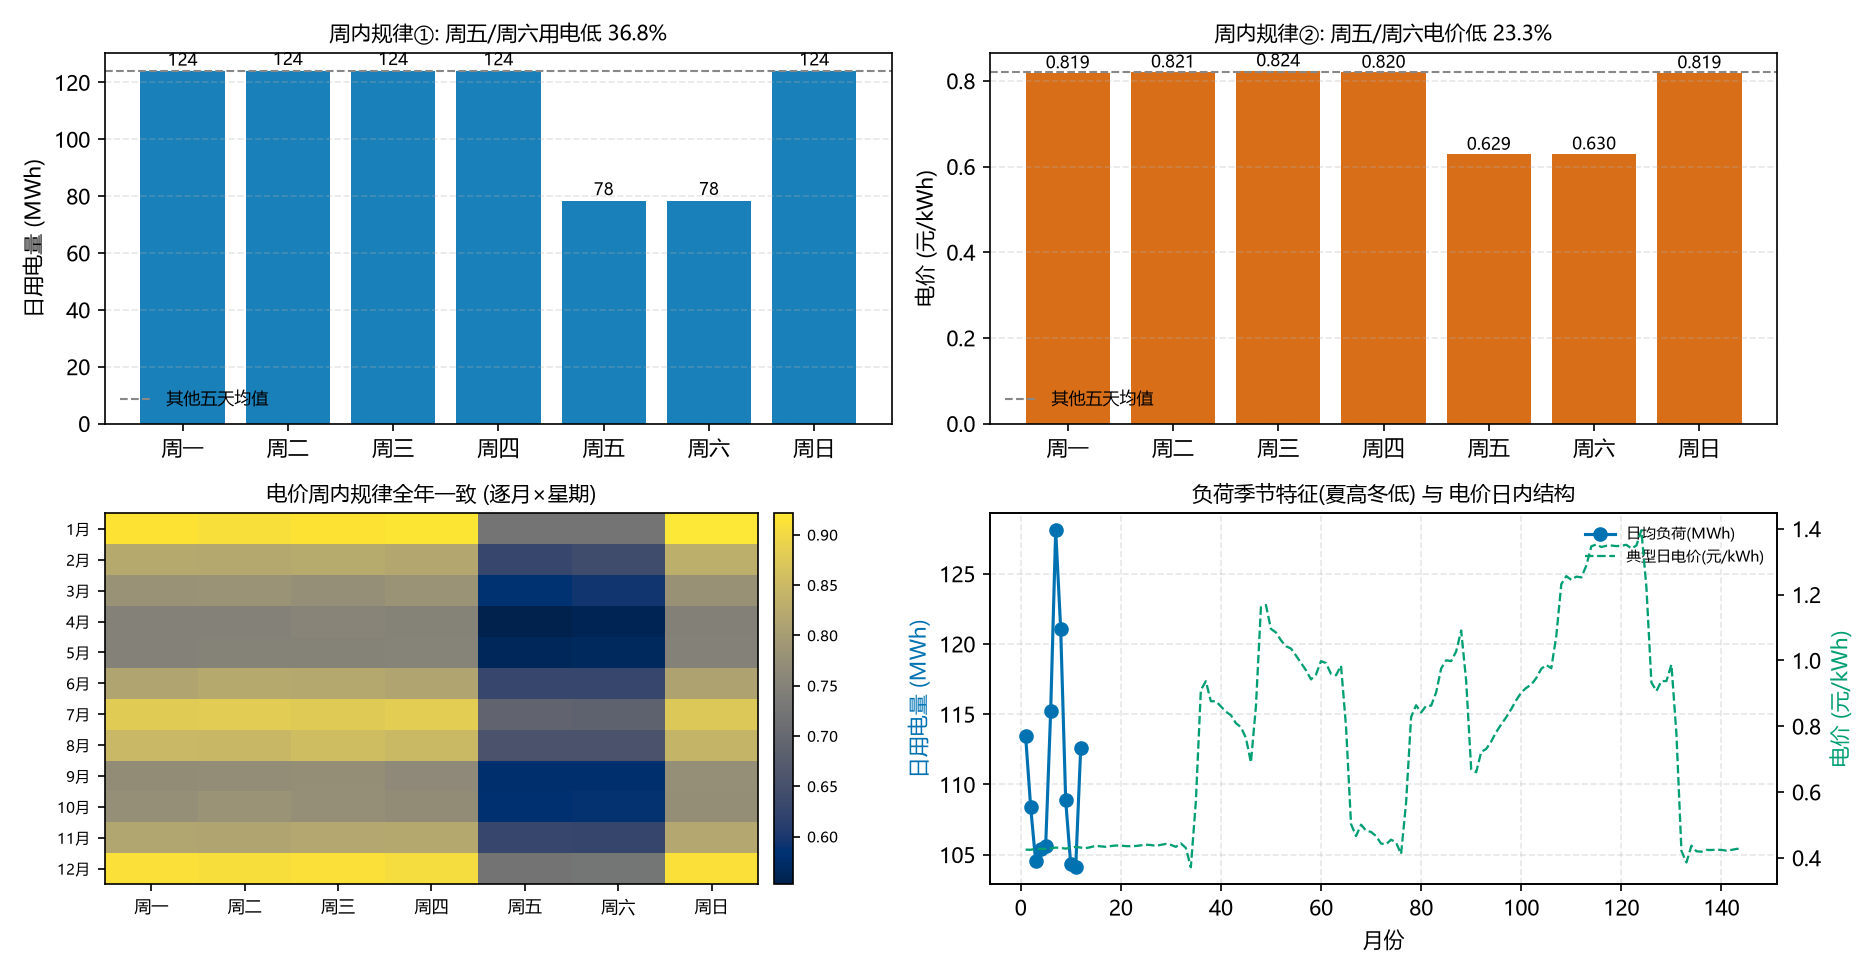
\includegraphics[width=0.92\textwidth]{figures/fig_weekly.png}
\caption{周内规律\nobreak：日均用电量（左上\nobreak）\nobreak、日均电价（右上\nobreak）\nobreak、逐月$\times$星期电价热力图（左下\nobreak）\nobreak、
负荷季节特征与电价日内结构（右下\nobreak）}
\label{fig:weekly}
\end{figure}

\begin{figure}[htbp]
\centering
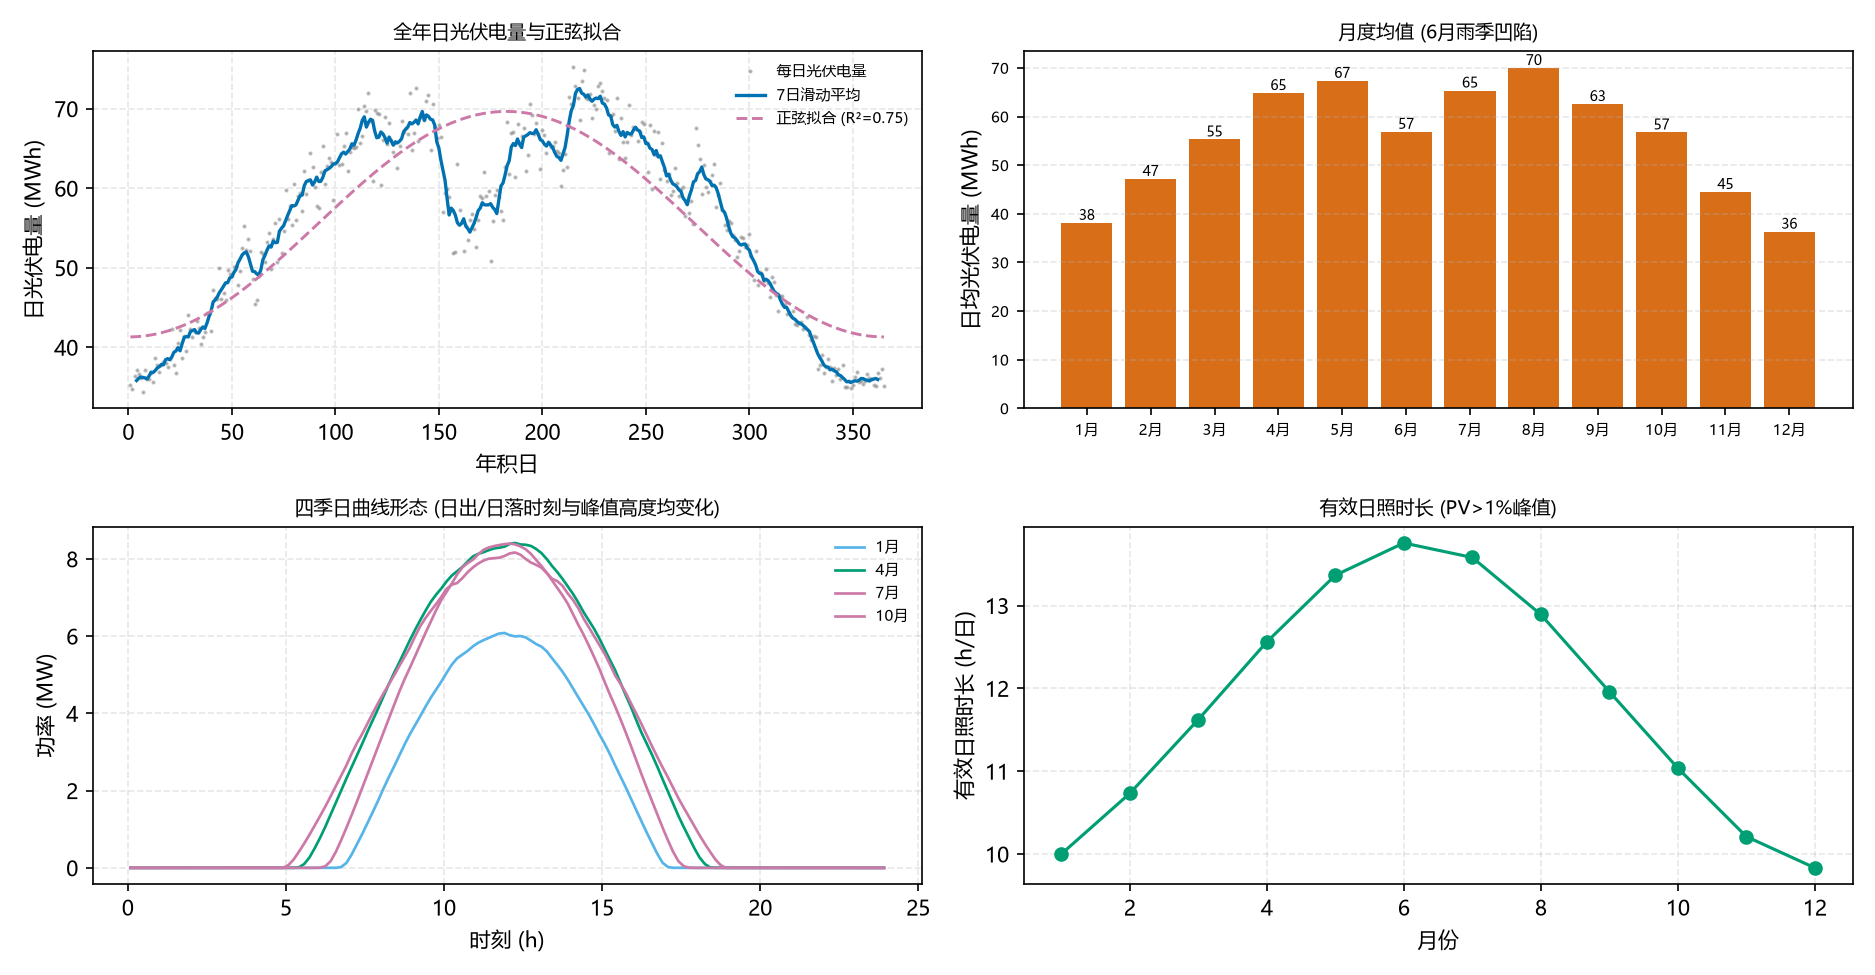
\includegraphics[width=0.92\textwidth]{figures/fig_pv_season.png}
\caption{光伏季节特征\nobreak：全年日电量与正弦拟合（左上\nobreak）\nobreak、月度均值与雨季凹陷（右上\nobreak）\nobreak、
四季日曲线形态（左下\nobreak）\nobreak、有效日照时长（右下\nobreak）}
\label{fig:pvseason}
\end{figure}

\subsection{规律四\nobreak：光伏与负荷噪声的重尾特征}

以“近 4 个同类日平均/近 4 日均值\nobreak”为基值\nobreak，净需求残差 $e=e_L-e_P$ 的分布呈现明显
\textbf{重尾}\nobreak：偏度均值 $+0.16$（近似对称\nobreak）\nobreak，而\textbf{超额峰度均值 $+5.96$}（正态为 0\nobreak，
个别时段高达 21\nobreak）\nobreak；标准差最大出现在 12 时（112.2 kWh/时段\nobreak）\nobreak，与正午光伏波动一致\nobreak。
按月看\nobreak，光伏基值误差的标准差在春季与雨季最大（MAE 31--35 kWh/时段\nobreak）\nobreak，12 月最小（12.9\nobreak）\nobreak。

\textbf{建模决策（已建模\nobreak：经验分位缓冲\nobreak；并证明“形式不重要\nobreak、水平才重要\nobreak”\nobreak）}\nobreak：安全裕度取
\textbf{近 30 天净残差的 70\% 经验分位}\nobreak。五组对照实验（\cref{tab:buffer}\nobreak）显示\nobreak：
各种更复杂的形式与本文方案的差异都在 $\pm0.6\text{\%}$ 以内
（分噪声叠加 $-0.52\text{\%}$\nobreak、正态参数化 $+0.58\text{\%}$\nobreak、60/90 天长窗 $+0.03$/$+0.16\text{\%}$\nobreak）\nobreak，
而\textbf{分位水平}偏离 0.7 的代价则大得多（$q=0.5$ 时 $+8.27\text{\%}$\nobreak，见第 \ref{sec:compare} 节\nobreak）\nobreak。
其中“分噪声叠加\nobreak”虽在全年上略优 0.52\%\nobreak，但它需要\textbf{分别估计负荷与光伏两个误差分布}
（受文献\cite{cqut253,cqut276}“分特征/分时建模\nobreak、误差不确定性显式计入调度\nobreak”思想启发\nobreak）\nobreak，
参数更多\nobreak，且对\textbf{净需求}的报童问题而言\nobreak，理论上正确的量正是净残差分位\nobreak；
本文保留最简且理论更直接的净残差经验分位\nobreak，把分噪声估计列入第 10 节的改进方向\nobreak。

\begin{table}[htbp]
\centering
\caption{安全裕度（缓冲\nobreak）方案的对照实验（全年 2.1--12.31 购电总费用\nobreak）}
\label{tab:buffer}
\zihao{-5}
\begin{tabular}{@{}lccc@{}}
\toprule
缓冲方案 & 全年总费用(元) & 相对采用 & 结论 \\
\midrule
\textbf{近30天净残差经验分位 $q^*=0.7$（采用\nobreak）} & \textbf{13\,655\,835} & --- & 最简形式\nobreak、理论直接 \\
负荷/光伏噪声分别取分位后叠加 & 13\,585\,138 & $-70\,697$ & 参数更多\nobreak，事后择优 \\
正态参数化（按小时 $\sigma$\nobreak，$z_{0.7}$\nobreak） & 13\,734\,664 & $+78\,829$ & 重尾欠覆盖 \\
净残差经验分位（60 天窗\nobreak） & 13\,659\,929 & $+4\,094$ & 信息陈旧 \\
净残差经验分位（90 天窗\nobreak） & 13\,677\,410 & $+21\,575$ & 信息陈旧 \\
\bottomrule
\end{tabular}
\end{table}

\subsection{规律五\nobreak：预测信息价值分解（预言机分析\nobreak）}

为进一步判断“是否值得为预测噪声投入更复杂的模型\nobreak”\nobreak，本文设计\textbf{预言机（oracle\nobreak）分解}\nobreak：
分别构造“光伏完全已知\nobreak”（$PV$ 用实测值\nobreak，负载仍用预测\nobreak）与“负载完全已知\nobreak”（负载用实测值\nobreak，
光伏仍用预测\nobreak）两个反事实链条\nobreak，与采用方案\nobreak、完全信息下界比较（\cref{fig:noise}\nobreak）\nobreak：

\begin{equation}
\begin{aligned}
\underbrace{13\,655\,835}_{\text{采用方案}}
&\xrightarrow[\text{光伏噪声价值 }491\,182]{}
\underbrace{13\,164\,653}_{PV\text{完美}},\\
\underbrace{13\,655\,835}_{\text{采用方案}}
&\xrightarrow[\text{负荷噪声价值 }423\,973]{}
\underbrace{13\,231\,862}_{L\text{完美}},\\
&\underbrace{12\,286\,531}_{\text{完全信息下界}} .
\end{aligned}
\end{equation}

即距完全信息下界的 136.9 万元缺口主要由三部分构成\nobreak：\textbf{光伏噪声 49.1 万元（35.9\%\nobreak）\nobreak、
负荷噪声 42.4 万元（31.0\%\nobreak）\nobreak、交互项 33.2\%}\nobreak。
\textbf{建模决策}\nobreak：两项噪声的信息价值合计仅 91.5 万元（占总费用 6.7\%\nobreak）\nobreak，
而且这是“完美预知\nobreak”的\textbf{理论上限}\nobreak、不可实现\nobreak；作为对比\nobreak，本文的\textbf{实时平衡控制}
在同一条计划下就省下 90.2 万元（相对僵硬执行 $-6.20\text{\%}$\nobreak）\nobreak，与这一上限同量级\nobreak。
因此本文\textbf{不引入分布鲁棒优化\nobreak、机会约束等重装备}\nobreak，
而是按“先核算信息价值\nobreak、再决定建模投入\nobreak”的原则\nobreak，把建模资源投在\textbf{可实现的实时平衡控制}
与\textbf{低成本高收益的预测模型组合}上（第 \ref{sec:q2} 节\nobreak）\nobreak。

\subsection{规律六\nobreak：预报误差随提前期增长}

附件3 预报的平均绝对误差随提前期增大\nobreak：0:00 发布为 181.3 kW\nobreak，6:00 发布 97.4 kW\nobreak，
12:00 发布 208.1 kW\nobreak，18:00 发布 260.1 kW（\cref{fig:fcerr}\nobreak）\nobreak；同一目标小时在相邻 6 小时
两次预报之间的平均修正幅度为 \textbf{273 kW}\nobreak。\textbf{建模决策（已建模\nobreak：滚动调整\nobreak，且必须“重新定裕度\nobreak”\nobreak）}\nobreak：
Q3 采用滚动时域调整（第~\ref{sec:q3} 节\nobreak）\nobreak。实测显示\nobreak，调整的价值\textbf{完全取决于“该时刻的预报
是否带来新信息\nobreak”以及“裕度是否随预报重新标定\nobreak”}——
\textbf{三个发布时刻全用（全滚动）值 116.6 万元}（13\,368\,415 元\nobreak，$-8.02\text{\%}$\nobreak）\nobreak，
而\textbf{单用 6:00/12:00/18:00 分别只值 42.4/78.4/86.0 万元}（14\,110\,726 / 13\,750\,895 / 13\,674\,623 元\nobreak）\nobreak，
两两组合（13\,620\,154 / 13\,503\,312 元\nobreak）仍不及全滚动\nobreak。
更关键的是\nobreak：若调整时\textbf{沿用 0:00 的旧裕度}而不按当日新预报重新标定残差分位\nobreak，
费用立刻升到 \textbf{13\,415\,035 元（比全滚动贵 4.66 万元\nobreak）}\nobreak，
说明\textbf{“调整了预报却不调整安全裕度\nobreak”会让调整彻底失效}（\cref{tab:q3cmp}\nobreak）\nobreak。
这与“预报在持续改进\nobreak”并不矛盾——预报改进的价值首先被更好的 0:00 计划与实时平衡吸收\nobreak，
调整只在“信息增量大 $+$ 裕度同步更新\nobreak”时才产生正收益\nobreak。

\begin{figure}[htbp]
\centering
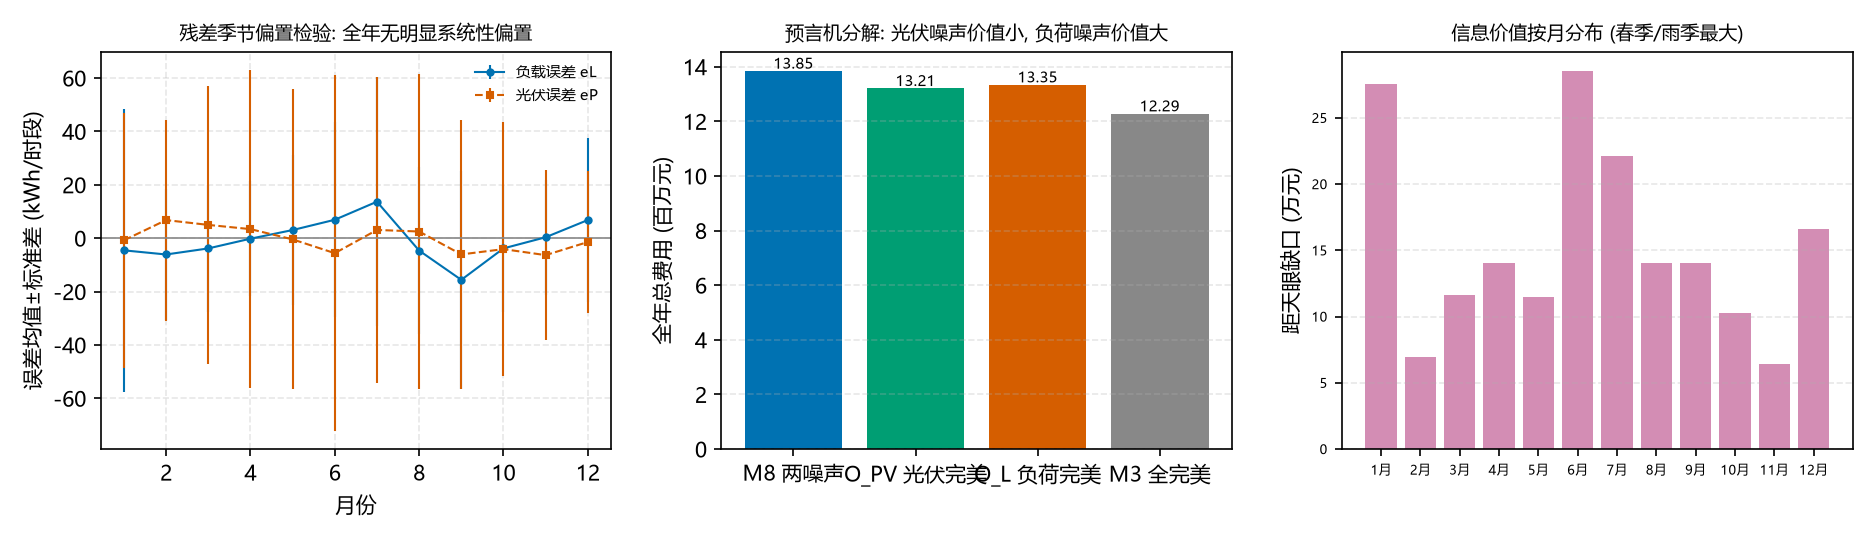
\includegraphics[width=0.95\textwidth]{figures/fig_noise.png}
\caption{噪声与季节性证据\nobreak：残差逐月均值$\pm$标准差（左\nobreak）\nobreak、预言机信息价值分解（中\nobreak）\nobreak、
距完全信息下界的缺口按月分布（右\nobreak）}
\label{fig:noise}
\end{figure}

\begin{figure}[htbp]
\centering
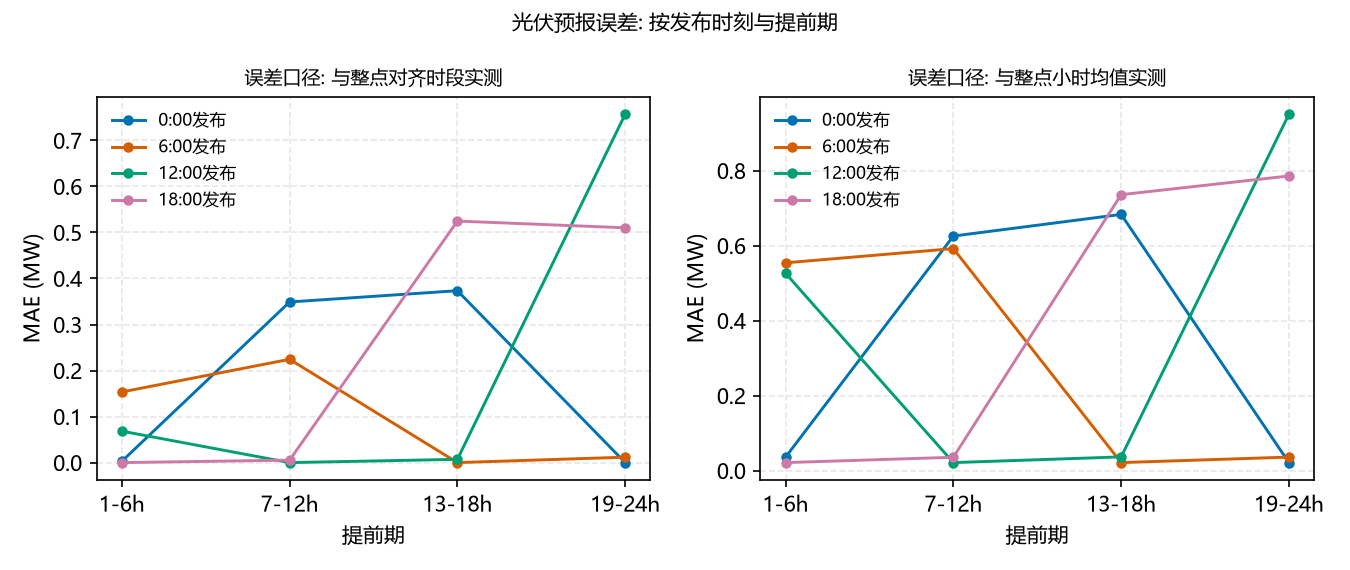
\includegraphics[width=0.85\textwidth]{figures/fig_fcerr.png}
\caption{光伏预报误差\nobreak：按发布时刻与提前期分桶的平均绝对误差}
\label{fig:fcerr}
\end{figure}

\subsection{规律与建模决策汇总}

\begin{table}[htbp]
\centering
\caption{全部数据规律及其建模决策}
\label{tab:patterns}
\zihao{-5}
\begin{tabularx}{\textwidth}{@{}p{2.5cm}p{3.6cm}p{2.4cm}X@{}}
\toprule
规律 & 关键数字 & 决策 & 依据/证据 \\
\midrule
周内负荷 & 周五六低 36.8\% & \textbf{已建模并升级}（水平$\times$形状 + 分类凸组合\nobreak） & 负载 MAE $137.5\to132.3$ kW（周五六 $-8.0\%$\nobreak）\nobreak，全年 $-36.5\text{\%}$ \\
周内电价 & 周五六低 23.3\% & 不单独建模 & LP 自动利用（周五净充最高\nobreak）\nobreak；用预测电价反而 $-0.20\text{\%}$ \\
光伏季节 & 1.93 倍\nobreak，正弦 $R^2=0.754$\nobreak，6 月凹陷 & 不单独建模 & 动量修正 $+0.63\text{\%}$\nobreak；残差无季节偏置\nobreak；$q^*$ 逐月不变 \\
负荷季节 & 夏高冬低（104--128 MWh/日\nobreak） & 不单独建模 & 同类日平均残差无季节偏置 \\
噪声重尾 & 峰度 $+5.96$ & \textbf{已建模}（经验分位缓冲\nobreak） & 复杂缓冲形式差异 $<0.6\text{\%}$\nobreak；$q=0.5$ 则 $+8.27\text{\%}$ \\
信息价值 & 光伏 35.9\%/负荷 31.0\%/交互 33.2\% & 只做“可实现的改进\nobreak” & 两项噪声上限 91.5 万\nobreak，实时平衡已省 90.2 万 \\
预报提前期 & MAE 181$\to$260 kW\nobreak；更新 273 kW & \textbf{已建模}（滚动调整\nobreak） & 升级 0:00 依据后调整无正收益（$-28.5\sim+0.3$ 万元\nobreak） \\
\bottomrule
\end{tabularx}
\end{table}
